% =====================================================================
\chapter{Funciones trigonométricas, inversas y ecuaciones}
\label{tema:4}
% =====================================================================

Este tema estudia el seno, el coseno y la tangente como funciones de una variable real: su periodicidad, sus gráficas y las transformaciones que producen las sinusoides generales. Después restringe sus dominios para obtener funciones inversas y, con ellas, describe todas las soluciones de las ecuaciones trigonométricas. Se sigue el capítulo~8 de~\cite{osat} (§8.1 a §8.3) y la §9.5 del mismo libro; la conexión con la codificación de la posición procede de Vaswani \emph{et al.}~\cite[§3.5]{vaswani}.

\section{Funciones periódicas}

\begin{definicion}[Función periódica]
Una función $f\colon D\to\R$ es \emph{periódica} de periodo $T>0$ si, para todo $x\in D$, se cumple $x+T\in D$, $x-T\in D$ y $f(x+T)=f(x)$. Si existe un periodo mínimo, se llama \emph{periodo fundamental}.
\end{definicion}

\begin{proposicion}\label{prop:periodos}
(i) El seno y el coseno tienen periodo fundamental $2\pi$; la tangente, $\pi$. (ii) Si $f$ tiene periodo fundamental $T$ y $\omega>0$, la función $g(x)=f(\omega x)$ tiene periodo fundamental $T/\omega$.
\end{proposicion}

\begin{proof}
(i) Por el \cref{teo:simetrias}(ii), $2\pi$ es periodo del seno y del coseno. Si $T>0$ es periodo del seno, $\sin(\frac{\pi}{2}+T)=\sin\frac{\pi}{2}=1$; el único punto de la circunferencia con ordenada~1 es $(0,1)=P(\pi/2)$, luego $P(\frac{\pi}{2}+T)=P(\frac{\pi}{2})$ y, por el \cref{teo:simetrias}(ii), $T\in2\pi\Z$, es decir, $T\ge2\pi$. Para el coseno se razona igual con $x=0$. Para la tangente, véase el \cref{eje:1-periodo-tan}. (ii) $g(x+T/\omega)=f(\omega x+T)=f(\omega x)=g(x)$. Si $0<S<T/\omega$ fuera periodo de $g$, entonces $f(y+\omega S)=g(\frac{y}{\omega}+S)=g(\frac{y}{\omega})=f(y)$ para todo $y$, y $\omega S<T$ sería periodo de $f$, contra la minimalidad de $T$.
\end{proof}

\section{Gráficas y sinusoides}

La \cref{fig:graficas} muestra las gráficas del seno y del coseno. Ambas oscilan entre $-1$ y $1$, y la del coseno es la del seno desplazada $\pi/2$ hacia la izquierda, porque $\cos x=\sin(x+\frac{\pi}{2})$ (\cref{teo:simetrias}(vi) con la paridad). La tangente tiene periodo $\pi$, ceros en $k\pi$ y asíntotas verticales en $\frac{\pi}{2}+k\pi$, donde se anula el coseno.

\begin{figure}[ht]
\centering
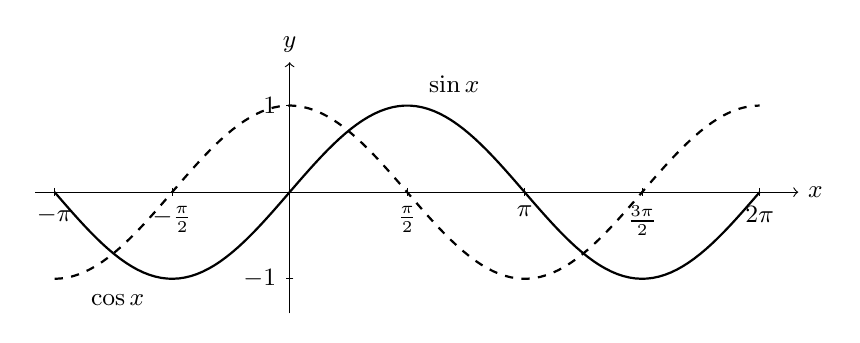
\begin{tikzpicture}[xscale=0.95,yscale=1.1,font=\small]
  \draw[->] (-3.4,0) -- (6.8,0) node[right] {$x$};
  \draw[->] (0,-1.4) -- (0,1.5) node[above] {$y$};
  \foreach \x/\l in {-3.1416/{-\pi},-1.5708/{-\frac{\pi}{2}},1.5708/{\frac{\pi}{2}},3.1416/{\pi},4.7124/{\frac{3\pi}{2}},6.2832/{2\pi}}
    \draw (\x,0.05) -- (\x,-0.05) node[below] {$\l$};
  \draw (0.05,1) -- (-0.05,1) node[left] {$1$};
  \draw (0.05,-1) -- (-0.05,-1) node[left] {$-1$};
  \draw[thick,domain=-3.1416:6.2832,samples=120] plot (\x,{sin(\x r)});
  \draw[thick,dashed,domain=-3.1416:6.2832,samples=120] plot (\x,{cos(\x r)});
  \node at (2.2,1.25) {$\sin x$};
  \node at (-2.3,-1.25) {$\cos x$};
\end{tikzpicture}
\caption{Gráficas de $\sin x$ (trazo continuo) y $\cos x$ (discontinuo) en $[-\pi,2\pi]$.}
\label{fig:graficas}
\end{figure}

\begin{definicion}[Sinusoide]
Una \emph{sinusoide} es una función $y=A\sin\bigl(\omega(x-x_0)\bigr)+D$ con $A\ne0$ y $\omega>0$. Se llaman \emph{amplitud} a $\abs{A}$, \emph{periodo} a $2\pi/\omega$, \emph{frecuencia angular} a $\omega$, \emph{desfase} (desplazamiento horizontal) a $x_0$ y \emph{desplazamiento vertical} a $D$.
\end{definicion}

Por la \cref{prop:periodos}(ii), el periodo de la sinusoide es efectivamente $2\pi/\omega$. Al escribir $y=A\sin(\omega x-c)+D$, el desfase es $x_0=c/\omega$, no $c$.

\begin{proposicion}[Suma de un seno y un coseno]\label{prop:armonico}
Sean $a,b\in\R$ no ambos nulos y $R=\sqrt{a^{2}+b^{2}}$. Existe $\varphi\in(-\pi,\pi]$ con $\cos\varphi=a/R$ y $\sin\varphi=b/R$, y para todo $x$
\[
a\sin x+b\cos x=R\sin(x+\varphi).
\]
En particular, el máximo de $a\sin x+b\cos x$ es $R$ y el mínimo, $-R$.
\end{proposicion}

\begin{proof}
El punto $(a/R,b/R)$ está en la circunferencia unidad, porque $(a^{2}+b^{2})/R^{2}=1$, luego es $P(\varphi)$ para algún $\varphi$, que puede tomarse en $(-\pi,\pi]$. Por el \cref{cor:suma}, $R\sin(x+\varphi)=R\sin x\cos\varphi+R\cos x\sin\varphi=a\sin x+b\cos x$. El valor extremo se sigue de que $\sin(x+\varphi)$ recorre $[-1,1]$.
\end{proof}

\section{Funciones trigonométricas inversas}

Una función periódica no es inyectiva, luego no tiene inversa. Se restringe a un intervalo donde sea biyectiva sobre su imagen~\cite[§8.3]{osat}.

\begin{definicion}[Inversas principales]\label{def:inversas}
\begin{enumerate}
  \item $\sin\colon[-\frac{\pi}{2},\frac{\pi}{2}]\to[-1,1]$ es biyectiva; su inversa es $\arcsin\colon[-1,1]\to[-\frac{\pi}{2},\frac{\pi}{2}]$.
  \item $\cos\colon[0,\pi]\to[-1,1]$ es biyectiva; su inversa es $\arccos\colon[-1,1]\to[0,\pi]$.
  \item $\tan\colon(-\frac{\pi}{2},\frac{\pi}{2})\to\R$ es biyectiva; su inversa es $\arctan\colon\R\to(-\frac{\pi}{2},\frac{\pi}{2})$.
\end{enumerate}
\end{definicion}

La inyectividad de estas restricciones se demuestra en el \cref{eje:4-creciente} (el seno es estrictamente creciente en $[-\frac{\pi}{2},\frac{\pi}{2}]$) y de forma análoga para las otras dos. La sobreyectividad es geométrica: cada recta horizontal $y=t$ con $\abs{t}\le1$ corta la semicircunferencia derecha en un punto, y cada recta vertical $x=t$ corta la superior en un punto; para la tangente, cada recta por el origen no vertical corta la semicircunferencia derecha abierta.

\begin{proposicion}[Propiedades de las inversas]\label{prop:inversas}
\begin{enumerate}
  \item $\sin(\arcsin x)=x$ para $x\in[-1,1]$, y $\arcsin(\sin\theta)=\theta$ si y solo si $\theta\in[-\frac{\pi}{2},\frac{\pi}{2}]$.
  \item $\cos(\arcsin x)=\sqrt{1-x^{2}}$ y $\sin(\arccos x)=\sqrt{1-x^{2}}$ para $x\in[-1,1]$.
  \item $\arcsin x+\arccos x=\frac{\pi}{2}$ para $x\in[-1,1]$.
  \item $\arcsin$ y $\arctan$ son impares, y $\arccos(-x)=\pi-\arccos x$.
\end{enumerate}
\end{proposicion}

\begin{proof}
(i) Es la definición de función inversa; si $\theta\notin[-\frac{\pi}{2},\frac{\pi}{2}]$, $\arcsin(\sin\theta)$ está en ese intervalo y no puede ser $\theta$. (ii) Sea $\theta=\arcsin x\in[-\frac{\pi}{2},\frac{\pi}{2}]$; ahí $\cos\theta\ge0$, luego $\cos\theta=+\sqrt{1-\sin^{2}\theta}=\sqrt{1-x^{2}}$. La segunda es análoga, con $\sin\ge0$ en $[0,\pi]$. (iii) Sea $\theta=\arcsin x$. Entonces $\frac{\pi}{2}-\theta\in[0,\pi]$ y $\cos(\frac{\pi}{2}-\theta)=\sin\theta=x$, luego $\arccos x=\frac{\pi}{2}-\theta$. (iv) Si $\theta=\arcsin x$, entonces $-\theta\in[-\frac{\pi}{2},\frac{\pi}{2}]$ y $\sin(-\theta)=-x$, luego $\arcsin(-x)=-\theta$; igual para $\arctan$. Si $\theta=\arccos x$, entonces $\pi-\theta\in[0,\pi]$ y $\cos(\pi-\theta)=-x$.
\end{proof}

\begin{ejemplo}\label{ej:inversas}
$\arcsin(\sin\frac{5\pi}{6})=\arcsin\frac12=\frac{\pi}{6}\ne\frac{5\pi}{6}$. Por la \cref{prop:inversas}(ii), $\cos(\arcsin\frac35)=\sqrt{1-\frac{9}{25}}=\frac45$.
\end{ejemplo}

\section{Ecuaciones trigonométricas}

\begin{teorema}[Soluciones generales]\label{teo:ecuaciones}
Sea $a\in\R$.
\begin{enumerate}
  \item Si $\abs{a}\le1$ y $\alpha=\arcsin a$, entonces $\sin x=a$ si y solo si $x=\alpha+2k\pi$ o $x=\pi-\alpha+2k\pi$ con $k\in\Z$.
  \item Si $\abs{a}\le1$ y $\beta=\arccos a$, entonces $\cos x=a$ si y solo si $x=\pm\beta+2k\pi$ con $k\in\Z$.
  \item Para todo $a$, $\tan x=a$ si y solo si $x=\arctan a+k\pi$ con $k\in\Z$.
\end{enumerate}
Si $\abs{a}>1$, las ecuaciones $\sin x=a$ y $\cos x=a$ no tienen solución.
\end{teorema}

\begin{proof}
(i) La recta $y=a$ corta la circunferencia unidad en los puntos $P(\alpha)$ y $P(\pi-\alpha)$, que tienen ordenada $a$ por el \cref{teo:simetrias}(iv), y en ningún otro (de $x^{2}=1-a^{2}$ salen a lo sumo dos abscisas, opuestas entre sí, y $P(\alpha)$, $P(\pi-\alpha)$ tienen abscisas $\cos\alpha$ y $-\cos\alpha$). Por tanto $\sin x=a$ si y solo si $P(x)\in\{P(\alpha),P(\pi-\alpha)\}$, y el \cref{teo:simetrias}(ii) traduce esta condición en la del enunciado. (ii) Igual, con la recta vertical $x=a$, que corta en $P(\beta)$ y $P(-\beta)$. (iii) La tangente tiene periodo $\pi$ y es inyectiva en $(-\frac{\pi}{2},\frac{\pi}{2})$; todo $x$ del dominio se escribe de forma única como $x=x_0+k\pi$ con $x_0$ en ese intervalo, y $\tan x=\tan x_0=a$ equivale a $x_0=\arctan a$. La última afirmación se debe a que $\abs{\sin x}\le1$ y $\abs{\cos x}\le1$.
\end{proof}

\begin{ejemplo}[Ecuación de segundo grado en el seno]\label{ej:cuadratica}
Para resolver $2\sin^{2}x+3\sin x+1=0$ en $[0,2\pi)$ se pone $s=\sin x$: $2s^{2}+3s+1=(2s+1)(s+1)=0$, de modo que $s=-\frac12$ o $s=-1$. Con el \cref{teo:ecuaciones}, $\sin x=-\frac12$ da $x=\frac{7\pi}{6}$ y $x=\frac{11\pi}{6}$, y $\sin x=-1$ da $x=\frac{3\pi}{2}$.
\end{ejemplo}

\begin{observacion}[Errores frecuentes]
(a) Dar solo $\arcsin a$ como solución de $\sin x=a$ y perder la familia $\pi-\arcsin a+2k\pi$. (b) Dividir ambos miembros por $\cos x$ o $\sin x$ sin estudiar aparte el caso en que se anulan: en $\sin2x=\cos x$ se pierden las soluciones con $\cos x=0$ (\cref{eje:4-doble}). (c) Elevar al cuadrado introduce soluciones falsas que deben descartarse sustituyendo (\cref{eje:4-cuadrado}). (d) Confundir el desfase $c$ de $\sin(\omega x-c)$ con el desplazamiento horizontal $c/\omega$.
\end{observacion}

\begin{observacion}[Conexión con el curso]
La codificación sinusoidal del Transformer~\cite[§3.5]{vaswani} asigna a la posición $p$ el vector con componentes $\PE(p)_{2i}=\sin(p\,\omega_i)$ y $\PE(p)_{2i+1}=\cos(p\,\omega_i)$, con frecuencias $\omega_i=10000^{-2i/d}$ (módulo~14, tema~4). Cada par de componentes es una sinusoide de la posición con periodo $2\pi/\omega_i$, y los periodos forman una progresión geométrica desde $2\pi$ hasta casi $2\pi\cdot10^{4}$. Las mismas frecuencias, con el nombre de longitudes de onda $\lambda_i=2\pi/\theta_i$, gobiernan la extensión del contexto de RoPE en el módulo~18 (tema~3).
\end{observacion}

\begin{lecturas}
\item OpenStax, \emph{Algebra and Trigonometry}~\cite{osat}, §8.1 «Graphs of the Sine and Cosine Functions», §8.2 «Graphs of the Other Trigonometric Functions», §8.3 «Inverse Trigonometric Functions» y §9.5 «Solving Trigonometric Equations».
\item Vaswani \emph{et al.}~\cite{vaswani}, §3.5 «Positional Encoding».
\end{lecturas}

\section*{Ejercicios del tema 4}
\addcontentsline{toc}{section}{Ejercicios del tema 4}

\begin{ejercicio}{1}{eje:4-parametros}
Para $y=3\sin(2x-\frac{\pi}{3})+1$, determine la amplitud, el periodo, el desplazamiento horizontal, el desplazamiento vertical y los valores máximo y mínimo.
\fuente{adaptado de OpenStax, \emph{Algebra and Trigonometry}~\cite{osat}, §8.1, ejercicios de la sección sobre amplitud, periodo y desfase.}
\end{ejercicio}

\begin{ejercicio}{1}{eje:4-dominios}
(a) Escriba el dominio y la imagen de $\arcsin$, $\arccos$ y $\arctan$, y explique por qué hay que restringir el dominio del seno antes de invertirlo. (b) Calcule $\arcsin(\sin\frac{3\pi}{4})$, $\arccos(\cos(-\frac{\pi}{3}))$ y $\tan(\arctan5)$.
\end{ejercicio}

\begin{ejercicio}{2}{eje:4-exactos}
Calcule el valor exacto de: (a)~$\arcsin(-\frac12)$; (b)~$\arccos(-\frac{\sqrt2}{2})$; (c)~$\arctan\sqrt3$; (d)~$\arccos(\cos\frac{5\pi}{3})$; (e)~$\sin(\arccos\frac35)$; (f)~$\tan(\arcsin\frac13)$.
\fuente{adaptado de OpenStax, \emph{Algebra and Trigonometry}~\cite{osat}, §8.3, ejercicios de la sección sobre evaluación y composición de inversas.}
\end{ejercicio}

\begin{ejercicio}{2}{eje:4-basicas}
Resuelva: (a) $2\sin x-1=0$, en $[0,2\pi)$ y en general; (b) $\tan x=-\sqrt3$, en general; (c) $\cos2x=\frac12$, en $[0,2\pi)$.
\fuente{adaptado de OpenStax, \emph{Algebra and Trigonometry}~\cite{osat}, §9.5, ejercicios de la sección sobre ecuaciones lineales en una función trigonométrica.}
\end{ejercicio}

\begin{ejercicio}{2}{eje:4-cuadratica}
Resuelva $2\cos^{2}x-\cos x-1=0$ en $\R$.
\fuente{adaptado de OpenStax, \emph{Algebra and Trigonometry}~\cite{osat}, §9.5, ejercicios de la sección sobre ecuaciones de tipo cuadrático.}
\end{ejercicio}

\begin{ejercicio}{2}{eje:4-doble}
Resuelva $\sin2x=\cos x$ en $[0,2\pi)$. Explique qué soluciones se perderían al dividir por $\cos x$.
\end{ejercicio}

\begin{ejercicio}{2}{eje:4-armonico}
Escriba $\sqrt3\sin x+\cos x$ en la forma $R\sin(x+\varphi)$, determine su máximo y dónde se alcanza en $[0,2\pi)$, y resuelva $\sqrt3\sin x+\cos x=1$ en $[0,2\pi)$.
\end{ejercicio}

\begin{ejercicio}{2}{eje:4-cuadrado}
Resuelva $\sin x+\cos x=1$ en $[0,2\pi)$ de dos maneras: (a) elevando al cuadrado y comprobando las soluciones obtenidas; (b) con la \cref{prop:armonico}. Explique por qué el método (a) produce soluciones falsas.
\end{ejercicio}

\begin{ejercicio}{2}{eje:4-periodo-suma}
Determine el periodo fundamental de $f(x)=\sin3x+\cos2x$ y de $g(x)=\sin^{2}x$. Para $f$, basta probar que $2\pi$ es periodo y que ningún $0<T<2\pi$ lo es; para esto último, estudie $f(T)$ y $f(-T)$ frente a $f(0)$.
\end{ejercicio}

\begin{ejercicio}{2}{eje:4-pe}
Sea $d=8$ y $\omega_i=10000^{-2i/d}$ para $i=0,1,2,3$. Calcule las cuatro frecuencias, los periodos $2\pi/\omega_i$ y el vector $\PE(1)\in\R^{8}$ con cuatro decimales. ¿Qué componentes distinguen bien las posiciones $1$ y $2$, y cuáles apenas cambian?
\fuente{definición de Vaswani \emph{et al.}~\cite[§3.5]{vaswani}; datos elegidos para el cálculo a mano.}
\end{ejercicio}

\begin{ejercicio}{3}{eje:4-creciente}
Demuestre que el seno es estrictamente creciente en $[-\frac{\pi}{2},\frac{\pi}{2}]$, y por tanto inyectivo en ese intervalo. Indicación: para $a>b$ en el intervalo, escriba $\sin a-\sin b$ como producto (\cref{cor:suma-producto}) y estudie el signo de cada factor.
\end{ejercicio}

\begin{ejercicio}{3}{eje:4-cos-iguales}
Demuestre que $\cos x=\cos y$ si y solo si $x=y+2k\pi$ o $x=-y+2k\pi$ para algún $k\in\Z$, usando la fórmula de $\cos x-\cos y$ como producto y el \cref{eje:1-periodo-tan}(a).
\end{ejercicio}

\begin{ejercicio}{3}{eje:4-arctan-inverso}
Demuestre que $\arctan x+\arctan\frac1x=\frac{\pi}{2}$ si $x>0$ y $-\frac{\pi}{2}$ si $x<0$.
\end{ejercicio}

\begin{ejercicio}{3}{eje:4-machin}
Demuestre que $\arctan\frac12+\arctan\frac13=\frac{\pi}{4}$. Justifique con cuidado por qué basta comprobar que la tangente de ambos miembros coincide.
\end{ejercicio}

\begin{ejercicio}{3}{eje:4-pe-lineal}
Sea $\omega>0$ y $v(p)=(\sin\omega p,\ \cos\omega p)\T$. Demuestre que para cada $k\in\R$ existe una matriz $M_k\in\R^{2\times2}$, que depende de $k$ y $\omega$ pero no de $p$, tal que $v(p+k)=M_kv(p)$ para todo $p$. Demuestre que $M_k$ es ortogonal ($M_k\T M_k=I$) y que $M_kM_l=M_{k+l}$.
\fuente{adaptado de la propiedad enunciada sin demostración por Vaswani \emph{et al.}~\cite[§3.5]{vaswani}.}
\end{ejercicio}
